% %%%%%%%%%%%%%%%%%%%%%%%%%%%%%%%%%%%%%%%%%%%%%%%%%%%%%%%%%%%%%%%%%%%%%%%%%%%%%%
% Start Preamble:
% %%%%%%%%%%%%%%%%%%%%%%%%%%%%%%%%%%%%%%%%%%%%%%%%%%%%%%%%%%%%%%%%%%%%%%%%%%%%%%

\documentclass[letterpaper,11pt,oneside,article]{memoir}\usepackage[]{graphicx}\usepackage[]{color}
%% maxwidth is the original width if it is less than linewidth
%% otherwise use linewidth (to make sure the graphics do not exceed the margin)
\makeatletter
\def\maxwidth{ %
  \ifdim\Gin@nat@width>\linewidth
    \linewidth
  \else
    \Gin@nat@width
  \fi
}
\makeatother

\definecolor{fgcolor}{rgb}{0.345, 0.345, 0.345}
\newcommand{\hlnum}[1]{\textcolor[rgb]{0.686,0.059,0.569}{#1}}%
\newcommand{\hlstr}[1]{\textcolor[rgb]{0.192,0.494,0.8}{#1}}%
\newcommand{\hlcom}[1]{\textcolor[rgb]{0.678,0.584,0.686}{\textit{#1}}}%
\newcommand{\hlopt}[1]{\textcolor[rgb]{0,0,0}{#1}}%
\newcommand{\hlstd}[1]{\textcolor[rgb]{0.345,0.345,0.345}{#1}}%
\newcommand{\hlkwa}[1]{\textcolor[rgb]{0.161,0.373,0.58}{\textbf{#1}}}%
\newcommand{\hlkwb}[1]{\textcolor[rgb]{0.69,0.353,0.396}{#1}}%
\newcommand{\hlkwc}[1]{\textcolor[rgb]{0.333,0.667,0.333}{#1}}%
\newcommand{\hlkwd}[1]{\textcolor[rgb]{0.737,0.353,0.396}{\textbf{#1}}}%

\usepackage{framed}
\makeatletter
\newenvironment{kframe}{%
 \def\at@end@of@kframe{}%
 \ifinner\ifhmode%
  \def\at@end@of@kframe{\end{minipage}}%
  \begin{minipage}{\columnwidth}%
 \fi\fi%
 \def\FrameCommand##1{\hskip\@totalleftmargin \hskip-\fboxsep
 \colorbox{shadecolor}{##1}\hskip-\fboxsep
     % There is no \\@totalrightmargin, so:
     \hskip-\linewidth \hskip-\@totalleftmargin \hskip\columnwidth}%
 \MakeFramed {\advance\hsize-\width
   \@totalleftmargin\z@ \linewidth\hsize
   \@setminipage}}%
 {\par\unskip\endMakeFramed%
 \at@end@of@kframe}
\makeatother

\definecolor{shadecolor}{rgb}{.97, .97, .97}
\definecolor{messagecolor}{rgb}{0, 0, 0}
\definecolor{warningcolor}{rgb}{1, 0, 1}
\definecolor{errorcolor}{rgb}{1, 0, 0}
\newenvironment{knitrout}{}{} % an empty environment to be redefined in TeX

\usepackage{alltt}

\setstocksize{279.4mm}{215.9mm}
\settrimmedsize{\stockheight}{\stockwidth}{*}
%\settypeblocksize{279.4mm}{*}{.65}
\setlrmarginsandblock{30mm}{60mm}{*}
%\setlength{\marginparwidth}{65mm}
\checkandfixthelayout

% These work nicely together for a work with lots of margin notes:
%\setlrmarginsandblock{30mm}{80mm}{*}
%\setmarginnotes{5mm}{65mm}{5mm}

\raggedbottom  % To avoid making LaTeX try to keep amount of
               % text vertically on page constant:

% To allow insertion of figures (jpeg, eps, etc..):
\usepackage{graphicx}
\setkeys{Gin}{width=\linewidth,totalheight=\textheight,keepaspectratio}
\graphicspath{{graphics/}}


\usepackage{ucs}        % Unicode (still needed?)
\usepackage[utf8x]{inputenc}   % Unicode (still needed?)
\usepackage{cancel}                       % For cancelling equations
\usepackage{helvet}
\usepackage{booktabs}  % Pretty tables
\usepackage{units} % The units package provides nice, non-stacked
                   % fractions and better spacing for units.
%\usepackage{multirow}   % Allows columns to span multiple
                         % rows in {tabular} environment
\usepackage{amssymb}
\usepackage{amsmath} % To allow complex math symbols
\usepackage{wrapfig}
\usepackage{hyperref}
\usepackage{lineno}

\usepackage{tikz}
\tikzstyle{ov}=[shape=rectangle,
                 draw=black!80,
                 minimum height=0.75cm,
                 minimum width=1cm,
                 thick]

\tikzstyle{av}=[shape=rectangle,
                 draw=black!80,
                 fill=black!10,
                 minimum height=1cm,
                 minimum width=1cm,
                 thick]

\tikzstyle{lv}=[shape=circle,
                  draw=black!80,
                  thick,
                  minimum width=1.5cm]
\usepackage{natbib} % For citations


\title{Dengue Dynamics}
\author{Krzysztof Sakrejda}
\date{\today}  % if the \date{} command is left out, current date will be used


% %%%%%%%%%%%%%%%%%%%%%%%%%%%%%%%%%%%%%%%%%%%%%%%%%%%%%%%%%%%%%%%%%%%%%%%%%%%%%%
% End Preamble
% %%%%%%%%%%%%%%%%%%%%%%%%%%%%%%%%%%%%%%%%%%%%%%%%%%%%%%%%%%%%%%%%%%%%%%%%%%%%%%
\IfFileExists{upquote.sty}{\usepackage{upquote}}{}
\begin{document}
\maketitle % this prints the handout title, author, and date
\begin{abstract}
Motivation:
\begin{enumerate}
\item VAR(p) form a basic class of models used for prediction in multiple
contexts (econometric tradition, ecology).  
\item After fitting, VAR(p) models are often analyzed for stability
(econometric, population biology cites) via a variety of
Eigen-decomposition based numerical methods which produce information on
long-run growth (stationarity/nonstationarity/near-non-stationarity),
oscillations (imaginary eigenvalues), transient dynamics and dampening
or instability).   
\item An alternative view of these diagnostic numbers sees them as
meaningful parameters in a generative model.
\item This alternative view suggests that we could place weak priors on
these parameters and encourage models that produce stable numbers.
\item Such models could still be checked for fit and predictive performance
\item In public health such models could be made to match the expert expectations that
under certain conditions specific diseases either fade or grow
explosively (unless mediated by interventions).  
\item Models tuned based on these priors should be viewed as:
 - descriptive and predictive, encoding an expert-driven bias.
 - in live prediction exercises, comparing biased model predictions to
   data is particularly critical to indicate when a model fails to
   capture unusual features (those that go against regularizing priors).
\end{enumerate}

Methods:
\begin{enumerate}
\item VAR(p) models can be re-written as VAR(1) models with a structured
projection matrix of coefficients, identity sub-matrices, and zero
sub-matrtices.
\item Eigenvalue decomposition of the fitted matrix can be used
diagnostically to indicate whether the fitted model represents a
stationary system, how fast the stationary system will return to
equilibrium after a disturbance, how strong the tendency to oscillate 
is, what periodicity/ies of oscillations is/are important.  These
features are used diagnostically after fitting a VAR(p) model to data.
\item Knowledge of infectious disease dynamics can also be encoded using 
the metrics derived from the components of an Eigenvalue decomposition.
For example infectious disease systems are known to be at least weak
stationary in endemic settings and nearly non-stationary models \emph{can} be
used to model hyperendemic settings.
\item We translate a series of [specific statements] on endemic and
hyperendemic infectious disease time series behavior into priors on
components of the Eigenvalue decomposition of a projection matrix.  
\item We characterize outputs of prior simulations based on reconstructing
the projection matrix from these prior components.
\item We fit VAR(p) models to simulated time series including seasonal, stationary,
and nearly non-stationary series.
\item We fit VAR(p) models to dengue data, we incorporate a reporting delay
model, we compare predictions to SPAMD/prior-unconstrained
SARIMA/frequentist SARIMA/MOA
\end{enumerate}
\end{abstract}


% %%%%%%%%%%%%%%%%%%%%%%%%%%%%%%%%%%%%%%%%%%%%%%%%%%%%%%%%%%%%%%%%%%%%%%%%%%%%%%
% Chapters:
% %%%%%%%%%%%%%%%%%%%%%%%%%%%%%%%%%%%%%%%%%%%%%%%%%%%%%%%%%%%%%%%%%%%%%%%%%%%%%%
%\begin{Spacing}{2}
%\linenumbers

% knitr preliminaries
\begin{knitrout}
\definecolor{shadecolor}{rgb}{0.969, 0.969, 0.969}\color{fgcolor}\begin{kframe}
\begin{alltt}
\hlkwd{library}\hlstd{(knitr)}
\hlkwd{read_chunk}\hlstd{(}\hlkwd{file.path}\hlstd{(R_dir,}\hlstr{'shared_data.R'}\hlstd{))}
\hlkwd{read_chunk}\hlstd{(}\hlkwd{file.path}\hlstd{(R_dir,}\hlstr{'approximation-plot.R'}\hlstd{))}
\end{alltt}
\end{kframe}
\end{knitrout}

\begin{knitrout}
\definecolor{shadecolor}{rgb}{0.969, 0.969, 0.969}\color{fgcolor}\begin{kframe}
\begin{alltt}
\hlkwd{library}\hlstd{(grid)}
\hlkwd{library}\hlstd{(ggplot2)}
\hlkwd{library}\hlstd{(dplyr)}
\hlkwd{library}\hlstd{(RPostgreSQL)}
\hlkwd{library}\hlstd{(integrator)}
\hlkwd{library}\hlstd{(cruftery)}
\end{alltt}
\end{kframe}
\end{knitrout}

\begin{knitrout}
\definecolor{shadecolor}{rgb}{0.969, 0.969, 0.969}\color{fgcolor}\begin{kframe}
\begin{alltt}
\hlstd{link} \hlkwb{<-} \hlkwd{db_connector}\hlstd{(}\hlstr{'~/credentials/pgsql-pass-dengue-local-db.rds'}\hlstd{)}
\end{alltt}


{\ttfamily\noindent\color{warningcolor}{\#\# Warning: Was not able to allocate a new connection, returned\\\#\# connection has lost its previously pending result.}}\end{kframe}
\end{knitrout}

% Meat
\chapter{The SIR model can be restated to ignore susceptibles.}\label{chap:sir-nosusceptibles}
%\epigraph{}{ }

The SI model is a simplification of the SIR model for a disease where infectious individuals leave
the infectious pool after one time step.  

\section{SI case}
The SI model  can be stated as a pair of equations describing
the size of the susceptible (S) and infected (I) population at time $t$
in terms of the system state at time $t-1$ and three groups of parameters: 
1) $r_t$, which describes the infectiousness of the disease at time $t$;
2) $\alpha_1$, and $\alpha_2$ which describe how effectively the
infected interact with the susceptible population and how effectively
the susceptible population mixes with the infected population; and 3)
the error terms $\epsilon_t$ and $u_t$.  The model is stated in equation
\ref{eq:sir-basic}.

\begin{align}\label{eq:sir-basic}
I_t &= r_t I_{t-1}^{\alpha_1} S_{t-1}^{\alpha_2} \epsilon_{t} \\
S_t &= B_{t-d} + S_{t-1} - I_t + u_t
\end{align}

One of the difficulties of applying this model is that the state
variables are not observed directly.  Only a case count (C) is observed
which is related to the number infected at time $t$ through a reporting
fraction $\rho_t$ as $I_t = \rho_t C_t$.  For estimation and to
understand the confounding which results from these limited observations
it would be useful to state the model in terms of infected individuals
only, leaving aside the dynamics of the susceptible population.
According to CITE CITE CITE this can be accomplished.  First we begin
by shifting the susceptible equation one time step back and using it to 
replace the $S_{t-1}$ term in the infectious equation:

\begin{align}
I_t &= r_t I_{t-1}^{\alpha_1} 
	\left[
		B_{t-1-d} + S_{t-2} - I_{t-1} + u_{t-1}
	\right]^{\alpha_2} \epsilon_{t} \\
\end{align}

Now the only term left for susceptibles is $S_{t-2}$ which we can
replace by shifting the infectious equation back one time step and
isolating $S$ on one side.

\begin{align}
S_{t-1}^{\alpha_2} &= \frac{I_t}{r_t I_{t-1}^{\alpha_1} \epsilon_{t}} \\
\alpha_2 \log S_{t-1} &= \log I_t - \log r_t - \alpha_1 \log I_{t-1} - \log \epsilon_{t}  \\
\log S_{t-1} &= \frac{\log I_t - \log r_t - \alpha_1 \log I_{t-1} - \log \epsilon_{t}}{\alpha_2}  \\
\log S_{t-2} &= \frac{\log I_{t-1} - \log r_{t-1} - \alpha_1 \log I_{t-2} - \log \epsilon_{t-1}}{\alpha_2}
\end{align}

This new representation of $S$ refers only to lagged terms of $I$ and
parameters.  It can be exponentiated and used to replace $S_{t-2}$ in the infectious
equation.  

\begin{align}
I_t &= r_t I_{t-1}^{\alpha_1} 
	\left[
		B_{t-1-d} + \exp\left(
			\frac{\log I_{t-1} - \log r_{t-1} - \alpha_1 \log I_{t-2} - \log \epsilon_{t-1}}{\alpha_2}
		\right) - I_{t-1} + u_{t-1}
	\right]^{\alpha_2} \epsilon_{t} \\
\end{align}

Using the log of this equation can clarify the role of different terms:

\begin{align}
\log I_t &= \log r_t + \alpha_1 \log I_{t-1} + \\
				 &	\alpha_2 \log \left[
		B_{t-1-d} + \exp\left(
			\frac{\log I_{t-1} - \log r_{t-1} - \alpha_1 \log I_{t-2} - \log \epsilon_{t-1}}{\alpha_2}
		\right) - I_{t-1} + u_{t-1}
	\right] + \log \epsilon_{t}
\end{align}

The multiplicative error terms appear in log form everywhere so their
expectation will be zero.  In the exponentiated term the (log) ratio of
infected individuals in two previous time steps appears.  Though the
equation is stated in terms of infected counts it could equally be
stated using the reporting equation and case counts rather than true
counts. 

\section{Multi-strain non-interacting SI}
A similar transformation is also possible for a multi-strain SI model
with non-interacting strains.  In this case we need to keep track of
strain-specific susceptibility and infection, which we do by
subscripting with one bit per strain.  An individual susceptible to all
strains is denoted as $S_{0000}$ and an individual immune to all but
the third strain is denoted as $S_{1101}$.  An individual susceptible to
to the third strain but with unknown status with regards to all others
is denoted as $S_{xx0x}$.  This last notation refers to a sum:

\begin{align}
	S_{(0xxx),t} &= S_{(0000),t} + S_{(0100),t} + S_{(0010),t} + \\
							 &+ S_{(0001),t} + S_{(0110),t} + S_{(0011),t} + \\
							 &+ S_{(0101),t} + S_{(0111),t}
\end{align}

With this notation in hand we can write the dynamics equations following
the example of the SI model.  

\begin{align}\label{eq:sir-multistrain}
	I_{(1xxx),t} &= r_{1,t} I_{(1xxx),t-1}^{\alpha_1} S_{(0xxx),t-1}^{\alpha_2} \epsilon_{t} \\
	S_{(0xxx),t} &= B_{t-d} + S_{(0xxx),t-1} - I_{(1xxx),t} + u_t
\end{align}

As before, $I_t$ is observed---at least in serotype-specfic data---and
the goal is to substitute out $S_t$ in all equations.  Immediately we
notice that indexing by strain susceptibility in the case of
non-interacting strains does not affect equation structure and we can
recycle the solution from original single-strain case.

\begin{align}
	\log I_{(1xxx),t} &= \log r_{1,t} + \alpha_1 \log I_{(1xxx),t-1} + \\
				 &	\alpha_2 \log \left[
		B_{t-1-d} + \exp\left(
			\frac{\log I_{(1xxx),t-1} - \log r_{1,t-1} - \alpha_1 \log
			I_{(1xxx),t-2} - \log \epsilon_{t-1}}{\alpha_2}
		\right) - I_{(1xxx),t-1} + u_{t-1}
	\right] + \log \epsilon_{t}
\end{align}

Ultimately the change is trivial because there are no interactions and
we are monitoring an important state variable.  

\section{Multi-strain interacting SI}

As a next step, we introduce interactions into the multi-strain SI
model.  In this model the immune history of the individualis allowed to
affect the infection rate.  Due to this change we can no longer lump
all susceptible individuals together in a sum term which complicates the
process of removing susceptibles from the equation.  Conveniently, the
infected individuals still function only as a group regardless of their
previous infection status.

\begin{align}\label{eq:sir-interacting}
I_t &= r_t I_{t-1}^{\alpha_1} S_{t-1}^{\alpha_2} \epsilon_{t} \\
S_t &= B_{t-d} + S_{t-1} - I_t + u_t
\end{align}



%\input{observation-process.tex}

\chapter{A generic error structure for continuous-time dynamics.}

Real-time data commonly arrives with a variety of associated time
scales. Working with continuous time provides two key advantages
for model building.  Decisions about how to align varying time frames can be deferred
until later so that they do not drive the choice of model structure.


\section{Poisson process basics}

When describing a dynamical system we start with an arbitrary but smooth
intensity function which describes the instantenous rate of events
(e.g.- cases per day).  We are interested in producing a model for the
intensity function, written $\lambda(t)$, which describes this rate 
as a function of time.  

One obstacle we face is that we do not measure
the intensity directly, instead we measure the number of cases, $Y$,
arriving between time $s$ and time $t$.  To be exact we choose to use a  
half-open interval, $(s,t]$, to describe the period of time.  Using the
half-open interval simplifies future calculations and data preparation
by making it possible to combine intervals without calculating overlap
and to assign data unambiguously to intervals.  The complete notation
for a measurement is then $Y_{s,t,i}$ which indicates the count ($Y$),
the ends of the interval $(s,t)$, as well as an index for additioal 
covariates measured at the batch level.


\subsection{Homogenous Poisson process approximation}

In the standard application of the homogenous Poisson process, the
parameter, $m$, for the Poisson distribution can be 
calculated as the product of the fixed rate, $\lambda_i$ for batch $i$, and the
duration of time $t-s$.  This is can be thought of as a Poisson
regression where $t-s$ functions as the exposure adjustment. If $\lambda$ is 
allowed to vary by batch, this can describe a time-varying process, but at the 
cost of discontinuities.

\begin{knitrout}
\definecolor{shadecolor}{rgb}{0.969, 0.969, 0.969}\color{fgcolor}\begin{kframe}
\begin{alltt}
\hlstd{time} \hlkwb{<-} \hlnum{1}\hlopt{:}\hlnum{10}
\hlstd{rate} \hlkwb{<-} \hlkwd{seq}\hlstd{(}\hlkwc{from}\hlstd{=}\hlnum{11}\hlstd{,} \hlkwc{to}\hlstd{=}\hlnum{20}\hlstd{,} \hlkwc{length.out}\hlstd{=}\hlkwd{length}\hlstd{(time))}
\hlstd{n_per_batch} \hlkwb{<-} \hlnum{5}
\hlstd{data} \hlkwb{<-} \hlkwd{data.frame}\hlstd{(}
        \hlkwc{time} \hlstd{=} \hlkwd{rep}\hlstd{(time,n_per_batch),}
        \hlkwc{rate} \hlstd{=} \hlkwd{rep}\hlstd{(rate,n_per_batch)}
\hlstd{)}
\hlstd{data[[}\hlstr{'count'}\hlstd{]]} \hlkwb{<-} \hlkwd{rpois}\hlstd{(}\hlkwc{n}\hlstd{=}\hlkwd{nrow}\hlstd{(data),} \hlkwc{lambda}\hlstd{=data[[}\hlstr{'rate'}\hlstd{]])}
\hlstd{data} \hlkwb{<-} \hlstd{data[}\hlkwd{order}\hlstd{(data[[}\hlstr{'time'}\hlstd{]]),]}

\hlstd{f} \hlkwb{<-} \hlkwa{function}\hlstd{(}\hlkwc{lambdas}\hlstd{) \{}
        \hlstd{data[[}\hlstr{'lambda'}\hlstd{]]} \hlkwb{<-} \hlstd{lambdas[data[[}\hlstr{'time'}\hlstd{]]]}
        \hlstd{ll} \hlkwb{<-} \hlkwd{sum}\hlstd{(}\hlkwd{dpois}\hlstd{(}\hlkwc{x}\hlstd{=data[[}\hlstr{'count'}\hlstd{]],} \hlkwc{lambda}\hlstd{=data[[}\hlstr{'lambda'}\hlstd{]],} \hlkwc{log}\hlstd{=}\hlnum{TRUE}\hlstd{))}
        \hlkwd{return}\hlstd{(}\hlopt{-}\hlstd{ll)}
\hlstd{\}}

\hlstd{optzd} \hlkwb{<-} \hlkwd{optim}\hlstd{(}
        \hlkwc{par} \hlstd{=} \hlnum{12}\hlopt{:}\hlnum{21}\hlstd{,}
        \hlkwc{fn} \hlstd{= f,} \hlkwc{gr}\hlstd{=}\hlkwa{NULL}\hlstd{,}
        \hlkwc{method} \hlstd{=} \hlkwd{c}\hlstd{(}\hlstr{"L-BFGS-B"}\hlstd{),}
        \hlkwc{lower}\hlstd{=}\hlnum{10}\hlopt{^-}\hlnum{10}\hlstd{,} \hlkwc{upper}\hlstd{=}\hlnum{50}
\hlstd{)}

\hlstd{g} \hlkwb{<-} \hlkwa{function}\hlstd{(}\hlkwc{t}\hlstd{) optzd[[}\hlstr{'par'}\hlstd{]][}\hlkwd{floor}\hlstd{(t)}\hlopt{+}\hlnum{1}\hlstd{]}

\hlstd{ptzd} \hlkwb{<-} \hlkwd{data.frame}\hlstd{(}
        \hlkwc{x} \hlstd{=} \hlnum{0}\hlopt{:}\hlnum{9}\hlopt{+}\hlnum{.5}\hlstd{,}
        \hlkwc{y} \hlstd{=} \hlkwd{g}\hlstd{(}\hlnum{0}\hlopt{:}\hlnum{9}\hlopt{+}\hlnum{0.5}\hlstd{)}
\hlstd{)}

\hlkwd{library}\hlstd{(ggplot2)}
\hlstd{pl} \hlkwb{<-} \hlkwd{ggplot}\hlstd{(}
        \hlkwc{data}\hlstd{=data,}
        \hlkwd{aes}\hlstd{(}\hlkwc{x}\hlstd{=time}\hlopt{-}\hlnum{0.5}\hlstd{,} \hlkwc{y}\hlstd{=count)}
\hlstd{)} \hlopt{+} \hlkwd{geom_point}\hlstd{()} \hlopt{+}
                \hlkwd{geom_bar}\hlstd{(} \hlkwc{data}\hlstd{=ptzd,} \hlkwd{aes}\hlstd{(}\hlkwc{x}\hlstd{=x,}\hlkwc{y}\hlstd{=y),} \hlkwc{alpha}\hlstd{=}\hlnum{0.4}\hlstd{,} \hlkwc{stat}\hlstd{=}\hlstr{'identity'}\hlstd{)}
\end{alltt}
\end{kframe}
\end{knitrout}

\begin{knitrout}
\definecolor{shadecolor}{rgb}{0.969, 0.969, 0.969}\color{fgcolor}\begin{kframe}
\begin{alltt}
\hlkwd{saveRDS}\hlstd{(}\hlkwc{object}\hlstd{=pl,} \hlkwc{file}\hlstd{=}\hlkwd{file.path}\hlstd{(figure_dir,}\hlstr{'discrete-homo-poisson-process.rds'}\hlstd{))}
\end{alltt}
\end{kframe}
\end{knitrout}

\begin{knitrout}
\definecolor{shadecolor}{rgb}{0.969, 0.969, 0.969}\color{fgcolor}\begin{kframe}
\begin{alltt}
\hlstd{pl} \hlkwb{<-} \hlkwd{readRDS}\hlstd{(}\hlkwc{file}\hlstd{=}\hlkwd{file.path}\hlstd{(figure_dir,} \hlstr{'discrete-homo-poisson-process.rds'}\hlstd{))}
\hlkwd{print}\hlstd{(pl)}
\end{alltt}
\end{kframe}\begin{figure}[]

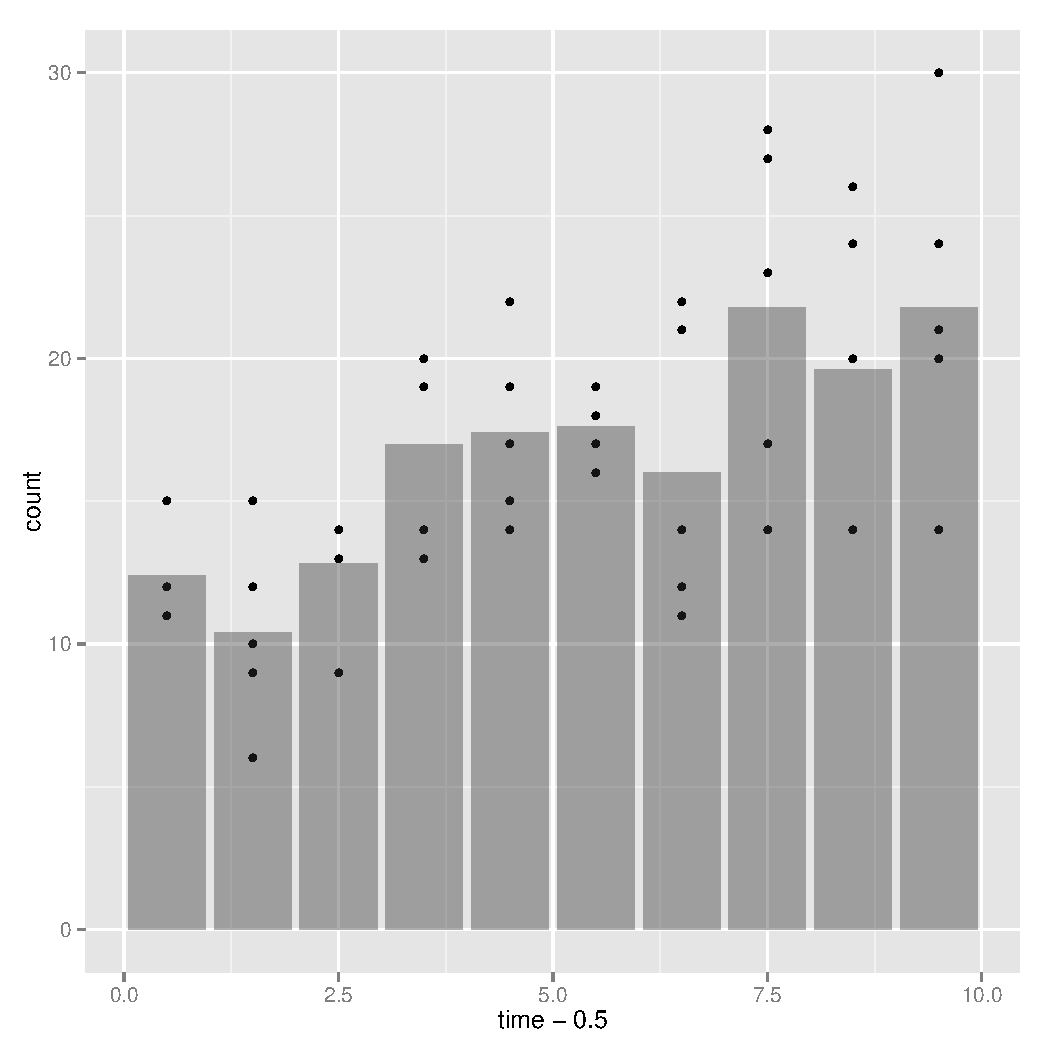
\includegraphics[width=\maxwidth]{figure/print-discrete-homo} \caption[Counts drawn from a Poisson distribution with time-varying rate]{Counts drawn from a Poisson distribution with time-varying rate.  Shaded areas describe the estimated probability mass function.  When boundaries between batches are biologically relevant this model is appropriate, but if boundaries are fluid the interpretability of the parameter at the boundary is limited.\label{fig:print-discrete-homo}}
\end{figure}


\end{knitrout}

As long as data is collected over well defined periods which match the
biological process being observed, the discontinuities are unimportant.
Sometimes, collection times vary and they may not be timed to changes in
the evolution of the biological process or the biological process may
be very dynamic as well as continuous which makes it difficult to time
data collection such that per-batch rate estimates are biologically
meaningful.  


\subsection{Inhomogenous Poisson process (IHPP)}

One way to avoid introducing the ambiguities that come with discrete
parameter batches is to use a continuous formulation of the Poisson
process which allows for a time-varying rate.  For any particular
count, $Y_{s,t,i}$, there is still a single paramter $m$, but now the
rate over the interval $(s,t]$ varies so we can no longer find the area, 
$m$, by multiplying the rate by the interval duration.  Instead we
define the intensity (or rate) function $\lambda(t)$ over the course
of the experiment.  To find the area $m_i(s,t)$ we use integration:

\begin{align}
	m_i(s,t) = \int_s^t \lambda_i(x)dx
\end{align}

Each count from a batch is still modeled as a Poisson distributed
random variable with parameter $m_i(s,t)$.  

\begin{knitrout}
\definecolor{shadecolor}{rgb}{0.969, 0.969, 0.969}\color{fgcolor}\begin{kframe}
\begin{alltt}
\hlkwd{library}\hlstd{(cruftery)}
\hlstd{data} \hlkwb{<-} \hlkwd{data.frame}\hlstd{(}
        \hlkwc{x}\hlstd{=}\hlkwd{seq}\hlstd{(}\hlkwc{from}\hlstd{=}\hlnum{0}\hlstd{,} \hlkwc{to}\hlstd{=}\hlnum{10}\hlstd{,} \hlkwc{length.out}\hlstd{=}\hlnum{10}\hlopt{^}\hlnum{3}\hlstd{),}
        \hlkwc{y}\hlstd{=}\hlkwd{gaussian_spline}\hlstd{(}\hlkwc{x}\hlstd{=}\hlkwd{seq}\hlstd{(}\hlkwc{from}\hlstd{=}\hlnum{0}\hlstd{,} \hlkwc{to}\hlstd{=}\hlnum{10}\hlstd{,} \hlkwc{length.out}\hlstd{=}\hlnum{10}\hlopt{^}\hlnum{3}\hlstd{),}
        \hlkwc{knot_points}\hlstd{=}\hlnum{2}\hlopt{:}\hlnum{8}\hlstd{,} \hlkwc{knot_weights}\hlstd{=}\hlkwd{exp}\hlstd{(}\hlkwd{rnorm}\hlstd{(}\hlnum{7}\hlstd{))}\hlopt{*}\hlnum{2}\hlopt{+}\hlkwd{c}\hlstd{(}\hlnum{0}\hlstd{,}\hlnum{2}\hlstd{,}\hlnum{2}\hlstd{,}\hlnum{2}\hlstd{,}\hlkwd{rep}\hlstd{(}\hlnum{0}\hlstd{,}\hlnum{3}\hlstd{)),} \hlkwc{knot_scale}\hlstd{=}\hlnum{0.5}\hlstd{)}
\hlstd{)}
\hlstd{shade} \hlkwb{<-} \hlstd{data[data[[}\hlstr{'x'}\hlstd{]]} \hlopt{>=} \hlnum{3} \hlopt{&} \hlstd{data[[}\hlstr{'x'}\hlstd{]]} \hlopt{<} \hlnum{5}\hlstd{,]}
\hlstd{shade} \hlkwb{<-} \hlkwd{rbind}\hlstd{(}
        \hlkwd{data.frame}\hlstd{(}\hlkwc{x}\hlstd{=}\hlnum{3}\hlstd{,}\hlkwc{y}\hlstd{=}\hlnum{0}\hlstd{),}
        \hlstd{shade,}
        \hlkwd{data.frame}\hlstd{(}\hlkwc{x}\hlstd{=}\hlnum{5}\hlstd{,}\hlkwc{y}\hlstd{=}\hlnum{0}\hlstd{)}
\hlstd{)}


\hlstd{pl} \hlkwb{<-} \hlkwd{ggplot}\hlstd{(}\hlkwc{data}\hlstd{=data,} \hlkwd{aes}\hlstd{(}\hlkwc{x}\hlstd{=x,} \hlkwc{y}\hlstd{=y))} \hlopt{+} \hlkwd{geom_line}\hlstd{()} \hlopt{+}
                        \hlkwd{geom_polygon}\hlstd{(}\hlkwc{data}\hlstd{=shade,} \hlkwd{aes}\hlstd{(}\hlkwc{x}\hlstd{=x,} \hlkwc{y}\hlstd{=y),} \hlkwc{alpha}\hlstd{=}\hlnum{0.3}\hlstd{)} \hlopt{+}
                        \hlkwd{xlab}\hlstd{(}\hlstr{'Time (days)'}\hlstd{)} \hlopt{+} \hlkwd{ylab}\hlstd{(}\hlstr{'Intensity (Cases per day)'}\hlstd{)} \hlopt{+}
                        \hlkwd{annotate}\hlstd{(}\hlstr{"text"}\hlstd{,} \hlkwc{x}\hlstd{=}\hlnum{3}\hlstd{,} \hlkwc{y}\hlstd{=}\hlopt{-}\hlnum{.2}\hlstd{,} \hlkwc{label}\hlstd{=}\hlstr{"s"}\hlstd{)} \hlopt{+}
                        \hlkwd{annotate}\hlstd{(}\hlstr{"text"}\hlstd{,} \hlkwc{x}\hlstd{=}\hlnum{5}\hlstd{,} \hlkwc{y}\hlstd{=}\hlopt{-}\hlnum{.2}\hlstd{,} \hlkwc{label}\hlstd{=}\hlstr{"t"}\hlstd{)} \hlopt{+}
                        \hlkwd{annotate}\hlstd{(}\hlstr{"text"}\hlstd{,} \hlkwc{x}\hlstd{=}\hlnum{4}\hlstd{,} \hlkwc{y}\hlstd{=} \hlnum{.8}\hlstd{,} \hlkwc{label}\hlstd{=}
                                \hlstr{"m(s,t)==integral(lambda(x)*dx,s,t)"}\hlstd{,} \hlkwc{parse}\hlstd{=}\hlnum{TRUE}\hlstd{)}
\end{alltt}
\end{kframe}
\end{knitrout}

\begin{knitrout}
\definecolor{shadecolor}{rgb}{0.969, 0.969, 0.969}\color{fgcolor}\begin{kframe}
\begin{alltt}
\hlkwd{saveRDS}\hlstd{(}\hlkwc{object}\hlstd{=pl,} \hlkwc{file}\hlstd{=}\hlkwd{file.path}\hlstd{(figure_dir,}\hlstr{'cont-inhomo-poisson-process.rds'}\hlstd{))}
\end{alltt}
\end{kframe}
\end{knitrout}

\begin{knitrout}
\definecolor{shadecolor}{rgb}{0.969, 0.969, 0.969}\color{fgcolor}\begin{kframe}
\begin{alltt}
\hlstd{pl} \hlkwb{<-} \hlkwd{readRDS}\hlstd{(}\hlkwc{file}\hlstd{=}\hlkwd{file.path}\hlstd{(figure_dir,} \hlstr{'cont-inhomo-poisson-process.rds'}\hlstd{))}
\hlkwd{print}\hlstd{(pl)}
\end{alltt}
\end{kframe}\begin{figure}[]

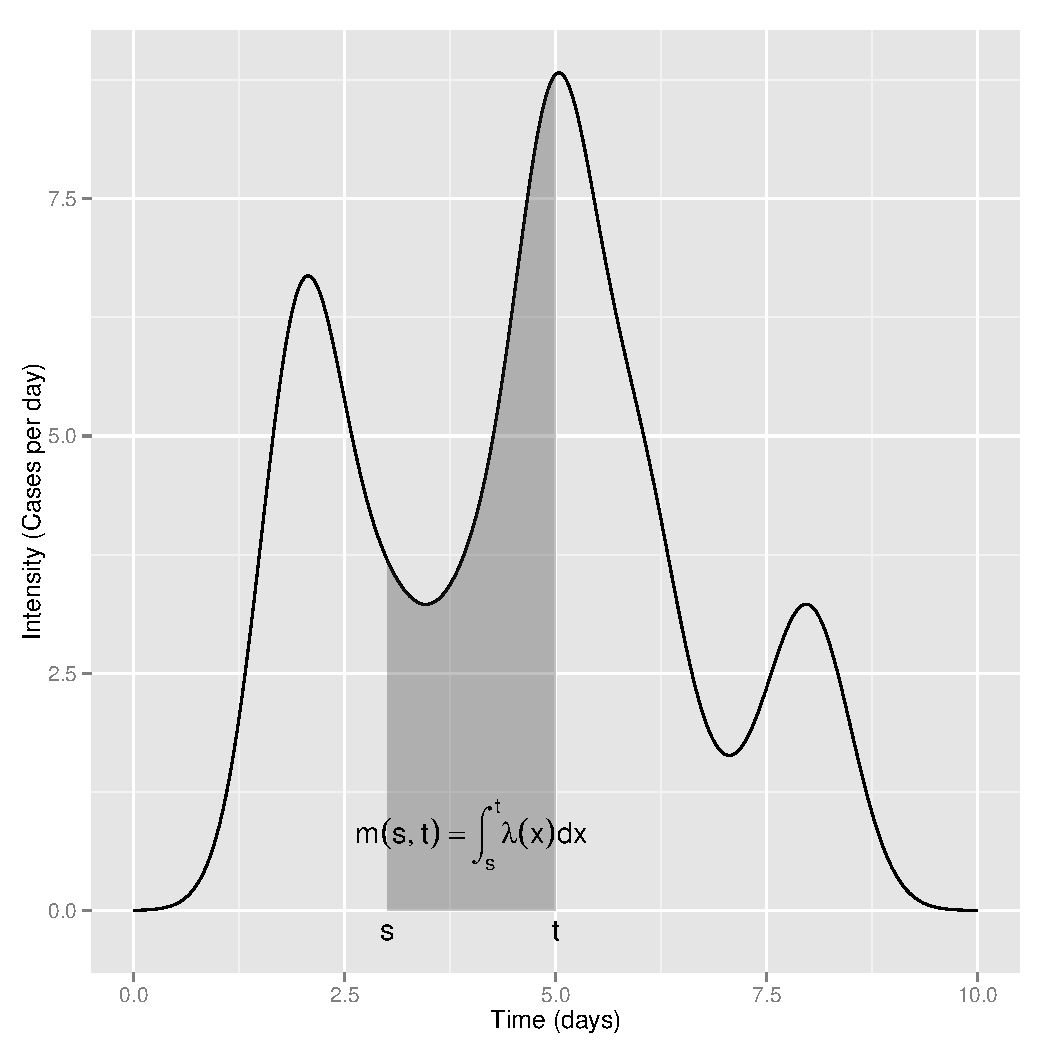
\includegraphics[width=\maxwidth]{figure/print-cont-inhomo} \caption[Counts drawn from a Poisson distribution with time-varying rate]{Counts drawn from a Poisson distribution with time-varying rate.  The curve is the intensity function in units of cases per day, which is integrated to give the Poisson distribution parameter.\label{fig:print-cont-inhomo}}
\end{figure}


\end{knitrout}

The inhomogenous poisson process makes an effective bridge between a
process conceptualized as continuous and real data collected on varying
time scales in a discrete fashion.  The focus of any further effort
can be on the function $\lambda(t)$ which is the rate of cases per
unit time.  The remaining difficulty is choosing a form of $\lambda(t)$
which is easy to integrate and allows us to apply the usual ameneties
of statistics---design matrices and linear models.

\section{Poisson process implementation}\label{sec:ihpp-implementation}

The two conditions on $\lambda(t)$ are that it should be easy to
integrate and that is should be amenable to further modeling.  For
this second reason, we choose to use a semiparameteric radial spline.
We spread $K$ knot points over the time period covered by the data
and use the normal distribution as a basis function.  The basis set is
then the set of normals centered on each knot point.  The function
$\lambda(t)$ then becomes a weighted sum of $K$ normals.

\begin{align}
\lambda(x) &= \sum_{k=1}^K \beta_k \frac{1}{\sqrt{2\pi}\sigma^2} \exp(\frac{1}{2\sigma^2}\left(x-\mu_k\right)^2)
\end{align}

This formulation allows us to further model the weights $\beta_k$ to
describe the effects relevant to a specific portion of time without
introducing discontinuities in the intensity function while still making
the function very flexible.  Formulating the intensity function as a sum
of normal densities also makes analytical integration possible as long
as the function has a known $CDF$.  Abusing notation slightly, the 
calculation of $m(s,t)$ becomes:

\begin{align}
m(s,t) &= \int_s^t \sum_{k=1}^K \beta_k PDF_N(x,\mu_k,\sigma^2) dx \\
			 &= \sum_{k=1}^K \beta_k \left(CDF_N(t,\mu_k,\sigma^2) - CDF_N(s,\mu_k,\sigma^2) \right)
\end{align}

Since calculations of many $CDF$'s, including the normal, are
efficiently coded in many libraries this is a generic strategy for
applying the IHPP to a variety of problems.  


















\chapter{Count data simulation for a continuous-time dynamics.}

For a simulation where the timing of events wihin batches is not
important but the number of events in a batch is important, it is
possible to avoid dealing with timing entirely and simply simulate
from the Poisson process conditional on $m(s,t)$ for each batch.
The key point for such a simulation becomes the calculation of $m(s,t)$.

To simulate event timing a thinning (rejection) algorithm is available which and
its efficiency depends on how well the proposed event distribution
matches the function $\lambda(t)$ as used for simulation or estimation.

\section{Splines for generating a smooth function}

To evaluate models constructed based on this Poisson process formulation
it will be important to have a way of simulating from the Poisson
process as described above and evaluating our ability to recover
parameters.  The appropriate splines and their integrals can be
constructed from a small set of R functions which implement the
calculations described in section \ref{sec:ihpp-implementation}.

\begin{knitrout}
\definecolor{shadecolor}{rgb}{0.969, 0.969, 0.969}\color{fgcolor}\begin{kframe}
\begin{alltt}
\hlkwd{read_chunk}\hlstd{(}\hlstr{'~/packages/cruftery/package_dir/R/spline_functions.R'}\hlstd{)}
\end{alltt}
\end{kframe}
\end{knitrout}

For any spline the function value at point x can be described as a
function of the basis function.  The rest of the calculations are
generic.

\begin{knitrout}
\definecolor{shadecolor}{rgb}{0.969, 0.969, 0.969}\color{fgcolor}\begin{kframe}
\begin{alltt}
\hlcom{# Generic radial spline:}
\hlstd{radial_spline} \hlkwb{<-} \hlkwa{function}\hlstd{(}\hlkwc{x}\hlstd{,} \hlkwc{f}\hlstd{,} \hlkwc{knot_points}\hlstd{,} \hlkwc{knot_weights}\hlstd{,} \hlkwc{knot_scale}\hlstd{) \{}
  \hlkwa{if} \hlstd{(}\hlkwd{length}\hlstd{(x)} \hlopt{==} \hlnum{1}\hlstd{) \{}
    \hlstd{knot_contributions} \hlkwb{<-} \hlkwd{f}\hlstd{(}\hlkwc{x}\hlstd{=x,} \hlkwc{center}\hlstd{=knot_points,} \hlkwc{scale}\hlstd{=knot_scale)}\hlopt{*}\hlstd{knot_weights}
    \hlkwd{return}\hlstd{(}\hlkwd{sum}\hlstd{(knot_contributions))}
  \hlstd{\}} \hlkwa{else} \hlstd{\{}
    \hlkwd{return}\hlstd{(}\hlkwd{sapply}\hlstd{(x,radial_spline,} \hlkwc{f}\hlstd{=f,} \hlkwc{knot_points}\hlstd{=knot_points,} \hlkwc{knot_weights}\hlstd{=knot_weights,} \hlkwc{knot_scale}\hlstd{=knot_scale))}
  \hlstd{\}}
\hlstd{\}}
\end{alltt}
\end{kframe}
\end{knitrout}

The generic spline function can be specialized for a gaussian spline
as follows.
\begin{knitrout}
\definecolor{shadecolor}{rgb}{0.969, 0.969, 0.969}\color{fgcolor}\begin{kframe}
\begin{alltt}
\hlcom{# Generic radial spline specialized to Gaussian.}
\hlstd{gaussian_spline} \hlkwb{<-} \hlkwa{function}\hlstd{(}\hlkwc{x}\hlstd{,} \hlkwc{knot_points}\hlstd{,} \hlkwc{knot_weights}\hlstd{,} \hlkwc{knot_scale}\hlstd{) \{}
  \hlstd{f} \hlkwb{<-} \hlkwa{function}\hlstd{(}\hlkwc{x}\hlstd{,} \hlkwc{center}\hlstd{,} \hlkwc{scale}\hlstd{)} \hlkwd{dnorm}\hlstd{(}\hlkwc{x}\hlstd{=x,} \hlkwc{mean}\hlstd{=center,} \hlkwc{sd}\hlstd{=scale)}
  \hlkwd{return}\hlstd{(}\hlkwd{radial_spline}\hlstd{(}\hlkwc{x}\hlstd{=x,} \hlkwc{f}\hlstd{=f,} \hlkwc{knot_points}\hlstd{=knot_points,} \hlkwc{knot_weights}\hlstd{=knot_weights,} \hlkwc{knot_scale}\hlstd{=knot_scale))}
\hlstd{\}}
\end{alltt}
\end{kframe}
\end{knitrout}

The integral can be coded in terms of R's CDF functions.
\begin{knitrout}
\definecolor{shadecolor}{rgb}{0.969, 0.969, 0.969}\color{fgcolor}\begin{kframe}
\begin{alltt}
\hlcom{# Integral of Gaussian radial spline.}
\hlstd{gaussian_spline_integral} \hlkwb{<-} \hlkwa{function}\hlstd{(}\hlkwc{knot_points}\hlstd{,} \hlkwc{knot_weights}\hlstd{,} \hlkwc{knot_scale}\hlstd{,} \hlkwc{a}\hlstd{,} \hlkwc{b}\hlstd{) \{}
  \hlstd{contributions} \hlkwb{<-} \hlkwd{mapply}\hlstd{(}
    \hlkwc{FUN}\hlstd{=}\hlkwa{function}\hlstd{(}\hlkwc{point}\hlstd{,} \hlkwc{weight}\hlstd{,} \hlkwc{scale}\hlstd{,} \hlkwc{a}\hlstd{,} \hlkwc{b}\hlstd{) \{}
      \hlstd{weight} \hlopt{*} \hlstd{(}\hlkwd{pnorm}\hlstd{(}\hlkwc{q}\hlstd{=b,} \hlkwc{mean}\hlstd{=point,} \hlkwc{sd}\hlstd{=scale)} \hlopt{-} \hlkwd{pnorm}\hlstd{(}\hlkwc{q}\hlstd{=a,} \hlkwc{mean}\hlstd{=point,} \hlkwc{sd}\hlstd{=scale))}
    \hlstd{\},}
    \hlkwc{point} \hlstd{= knot_points,} \hlkwc{weight} \hlstd{= knot_weights,}
    \hlkwc{MoreArgs} \hlstd{=} \hlkwd{list}\hlstd{(}\hlkwc{scale}\hlstd{=knot_scale,} \hlkwc{a}\hlstd{=a,} \hlkwc{b}\hlstd{=b)}
  \hlstd{)}
  \hlkwd{return}\hlstd{(}\hlkwd{sum}\hlstd{(contributions))}
\hlstd{\}}
\end{alltt}
\end{kframe}
\end{knitrout}

Given the spline integral function, it is simple to calculate $m(s,t)$
and simulate the number of events in a batch as:

\begin{align}
X \sim Poi(m(s,t)) 
\end{align}











\chapter{Reporting in the Poisson process context.}

\section{Modeling observed reporting data.}

The reporting delays, $t_d$, are observed.  These can be modelled
directly as, for example, having a weibull distribution.  To estimate
such a model we would:

\begin{enumerate}
\item load all data with the columns: \begin{itemize}
	\item $t_r$, the date of the report delivery.
	\item $t_s$, the date of illness.
	\item $t_d=t_r - t_s$, the reporting delay.
	\item $j$, the province.
	\end{itemize}
\end{enumerate}

Weibull model in Stan..., etc...

This lets us estimate parameter for a posterior density
$p(t_d|\theta_d)$.  

\section{The reporting problem in the Poisson process model.} 

The question we want to answer to integrate the reporting model with a
disease dynamics model is: 

Q1: What proportion of cases which occur between time point $t_a$ and
$t_b$ are reported by $t^*$.

Knowing this fraction, $f(t^*, t_a, t_b)$, would let us convert $y$, the
case count observed between time points $t_a$ and $t_b$, into $y^*$, the true (or reporting-adjusted) case
count.  

\begin{equation}
y = y^* \times f(t^*, t_a, t_b)
\end{equation}

It is likely that this is some kind of CDF for $t^*$, but it's
form is unclear. To get there we start by asserting that we will specify
two densities: one for the reporting/delay process and one for the
disease process:

\begin{align}
p_d(t_d|\theta_d) &= \ldots \\
p_s(t_s|\theta_s) &= \ldots
\end{align}

The disease process is a primary focus of this work and the poisson
process model can be used to estimate an intensity function as
described.  The density function for the dates of illness ($t_s$) is
(the same?) a transformation of the intensity function.

The reporting delays are directly observed and standard time-to-event
modeling techniques can be applied to estimate the parameters of the
density of $t_d$.  Due to the deterministic relationship between $t_r$
and $t_s$, we can specify a distribution for $t_r$ conditional on $t_s$.

\begin{equation}
p_r(t_r|\theta_d, t_s) = p_d(t_r - t_s| \theta_d) 
\end{equation}

To remove the conditionality on $t_s$, we can construct the joint
distribution for $p_{r,s}$ and integrate over the
possible values.  In the poisson process, counts are reported in batches
which begin at $a$ and end at $b$ restricting $t_a < t \le  t_b$,
and these are the relevant bounds for integration:

\begin{align}
p_{r,s}(t_r, t_s| \theta_d, \theta_s) = p_s(t_s|\theta_s) p_r(t_r|\theta_d, t_s) \\
p_r(t_r|\theta_d, \theta_s, a<t\le b) = \int_a^b p_s(t_s|\theta_s) p_r(t_r|\theta_d, t_s)
\end{align}

The resulting density is depends only on the parameters of the reporting
model ($\theta_d$), the disease model ($\theta_s$), and the boundaries
of the batch ($t \in [a,b)$).  This density defines the distribution of
reporting times for a batch of cases.  For cases to be available for a
model, they must be reported prior to, $t^*$,  the time of the analysis.  
The proportion of available cases can be stated in terms of the CDF: 

\begin{equation}
Pr[t_r < t^*| \theta_d, \theta_s, a<t\le b] = \int_a^{t^*} p_r(t_r|\theta_d, \theta_s, a<t<=b) dt_r
\end{equation}

Which lets us relate $y$ and $y^*$.

\begin{equation}
y = y^* \times Pr[t_r < t^*| \theta_d, \theta_s, a<t\le b]
\end{equation}

\section{Reasonable approximations to the rescue}

One difficulty with this approach is that we do not have an analytical
expression for $p_s$ (or its integral), which means we do not
have an analytical expression for $p_r$ (or its integral).  We begin
with an approximation of the disease process.  

First assume that $a$ and $b$ generate an interval short enough such
that $p_s$ is apprximately flat over this interval.  This requires that
counts for each batch are collected over a short period of time.  Then 

\begin{align}
t_s \sim U(a,b) \\
p(t_s|\theta_s, a^*, b^*) \sim \frac{1}{b^* - a^*}
\end{align}

If we also assume a Weibull distribution for the reporting
interval/delay, we can get an approximate density for $t_r$.

\begin{align}
p(t_r| \theta_d, t_s) &= k\lambda(t_d\lambda)^{k-1} e^{-(x\lambda)^k} \\
p(t_r| \theta_d, \theta_s, a < t_s \le  b) 
		&= \int_a^b p_s(t_s|\theta_s) p_r(t_r|\theta_d, t_s) dt_s\\
		&= \int_a^b \frac{1}{b^*-a^*} k\lambda(t_d\lambda)^{k-1} e^{-(t_d\lambda)^k} dt_s\\
		&= \frac{1}{b^*-a^*} \int_a^b \text{PDF}_{t_d}(t_r - t_s) dt_s\\
		&= \frac{1}{b^*-a^*} \big[ \text{CDF}_{t_d}(t_r-a|k,\lambda) - \text{CDF}_{t_d}(t_r-b|k,\lambda) \big]
\end{align}

Since the delays are in reverse-time, we flip integral bounds to get a positive
PDF function for $t_r$. Any model for $t_d$ which has an PDF with a
matching known CDF in closed form can be put through the same process.
The result is a scaled version of the original PDF with expanded
variance.



\begin{knitrout}
\definecolor{shadecolor}{rgb}{0.969, 0.969, 0.969}\color{fgcolor}\begin{kframe}
\begin{alltt}
\hlstd{pl} \hlkwb{<-} \hlkwd{readRDS}\hlstd{(}\hlkwc{file}\hlstd{=}\hlkwd{file.path}\hlstd{(figure_dir,} \hlstr{'reporting-approximation.rds'}\hlstd{))}
\hlkwd{print}\hlstd{(pl)}
\end{alltt}
\end{kframe}\begin{figure}[]

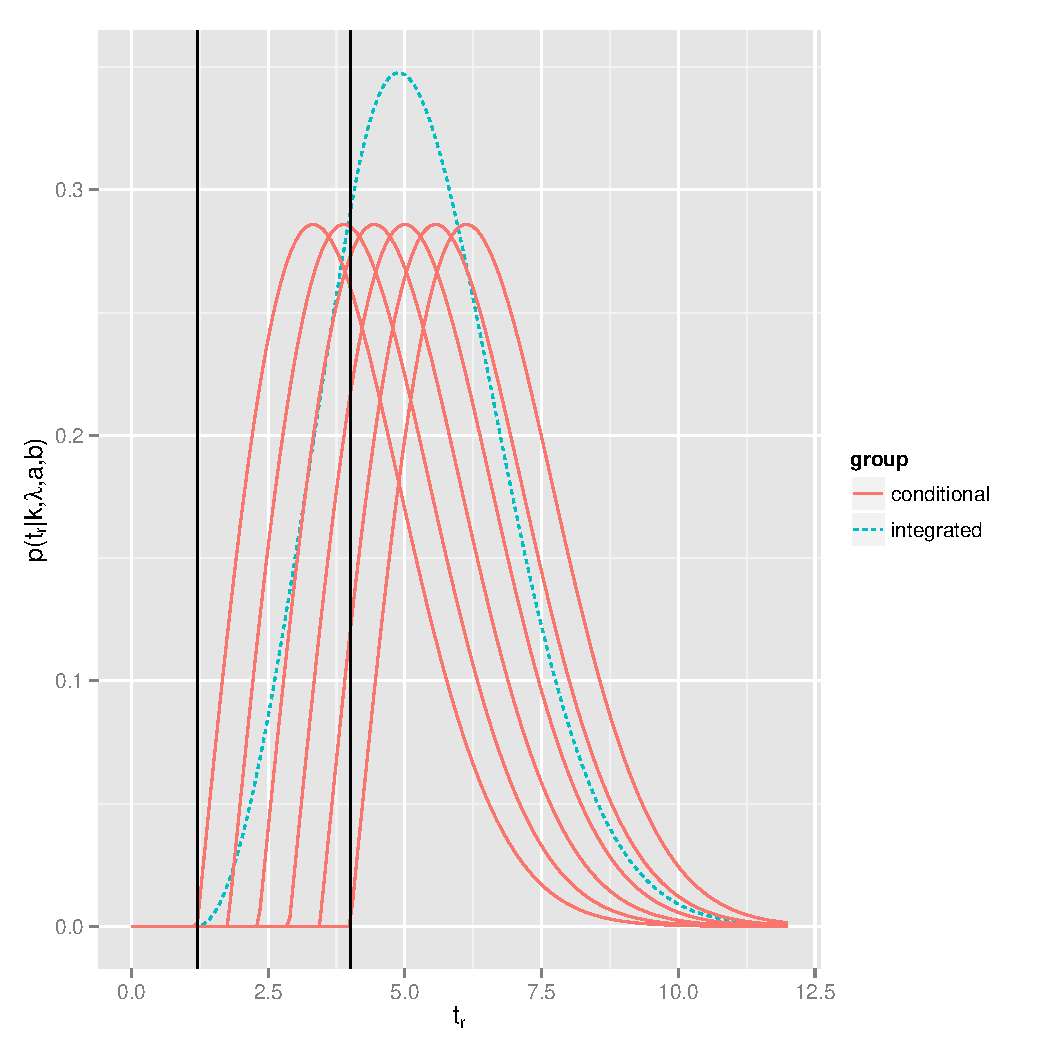
\includegraphics[width=\maxwidth]{figure/reporting-approximation-plot} \caption[Density for reporting dates, ($t_r$, shown with a dashed blue line), conditional on Weibull reporting delay distribution (shown in solid red lines) and bounds on the dates of illness ($a < t_s \le  b$, vertical lines)]{Density for reporting dates, ($t_r$, shown with a dashed blue line), conditional on Weibull reporting delay distribution (shown in solid red lines) and bounds on the dates of illness ($a < t_s \le  b$, vertical lines).\label{fig:reporting-approximation-plot}}
\end{figure}


\end{knitrout}

This gives us a closed-form solution for $t_r$, the density of reporting
times.  The final step is integrating this to get an expression for
$Pr[t_r < t^*| \theta_d, \theta_s, a<t\le b]$...

\begin{align}
Pr[&t_r < t^*| \theta_d, \theta_s, a<t\le b] =  \\
	&= \frac{1}{b^*-a^*} \Bigg[ 
		\int_a^{t^*} \text{CDF}_{t_d}(t_r-a|k,\lambda) - 
		\int_b^{t^*} \text{CDF}_{t_d}(t_r-b|k,\lambda) 
		\Bigg] \\
	&= \frac{1}{b^*-a^*} \Bigg[ 
		\int_a^{t^*} 1-e^{-([t_r-a]\lambda)^k} dt_r - \int_b^{t^*} 1-e^{-([t_r-b]\lambda)^k} dt_r 
	\Bigg] \\
	&= \frac{1}{b^*-a^*} \Bigg[ 
		\int_a^{t^*} 1 dt_r - \int_a^{t^*} e^{-([t_r-a]\lambda)^k} dt_r -
		\int_b^{t^*} 1 dt_r + \int_b^{t^*} e^{-([t_r-b]\lambda)^k} dt_r 
	\Bigg] \\
	&= \frac{1}{b^*-a^*} \Bigg[
		b - a +
		\int_a^{t^*} e^{-([t_r-a]\lambda)^k} dt_r +
		\int_b^{t^*} e^{-([t_r-b]\lambda)^k} dt_r 
	\Bigg] \\
\end{align}

The integrals can be rewritten in terms of incomplete upper gamma
functions.

\begin{align}
		\int_a^{t^*} & e^{-([t_r-a]\lambda)^k} dt_r = \\
			& \frac{(a-t^*)\Gamma(\frac{1}{k},[(t^*-a)\lambda]^k)}{(t^*-a)\lambda} -
			  \frac{(a-a  )\Gamma(\frac{1}{k},[(a  -a)\lambda]^k)}{ a  -a \lambda} = \\
			& -\frac{\Gamma(\frac{1}{k},[(t^*-a)\lambda]^k)}{\lambda} -
			  \frac{\Gamma(\frac{1}{k})}{\lambda} = \\
			& -\frac{1}{\lambda} \Bigg[
				\Gamma\bigg(\frac{1}{k},[(t^*-a)\lambda]^k\bigg) -
				\Gamma\bigg(\frac{1}{k}\bigg)
				\Bigg] = \\
			& \frac{1}{\lambda} \gamma\bigg(\frac{1}{k},\big[\lambda(t^*-a)\big]^k\bigg)
\end{align}

Which leaves the final expression as:

\begin{align}
Pr[&t_r < t^*| \theta_d, \theta_s, a<t\le b] =  \\
	&= \frac{1}{b^*-a^*} \Bigg[
		b - a +
		\int_a^{t^*} e^{-([t_r-a]\lambda)^k} dt_r +
		\int_b^{t^*} e^{-([t_r-b]\lambda)^k} dt_r 
	\Bigg] = \\
	&= \frac{1}{b^*-a^*} \Bigg[
		b - a + \frac{1}{\lambda} \bigg(
			\gamma\big(k^{-1},\big[\lambda(t^*-a)\big]^k\big) + 
			\gamma\big(k^{-1},\big[\lambda(t^*-b)\big]^k\big)
		\bigg)
	\Bigg]
\end{align}

This can be implemented in Stan for each instance of the incomplete
lower gamma function ($\gamma(a,x)$) by using the product of the normalized lower
incomplete gamma function (\verb#gamma_p#) and the gamma function
(\verb#tgamma#).  The equivalent is available in R and a more efficient 
method may be available (after all the outcome of this difference in
incomplete lower gamma functions is an integral over the scaled duration
of the interval during which the batch was reported).





% Extras
%\appendix
%\chapter{<Catchy title>}\label{chap:appendixA}
\section{<Quick and topical>}\label{sec:sectionA}
One example of the process of going from process... 



% Cruft


%\end{Spacing}
% %%%%%%%%%%%%%%%%%%%%%%%%%%%%%%%%%%%%%%%%%%%%%%%%%%%%%%%%%%%%%%%%%%%%%%%%%%%%%%




% %%%%%%%%%%%%%%%%%%%%%%%%%%%%%%%%%%%%%%%%%%%%%%%%%%%%%%%%%%%%%%%%%%%%%%%%%%%%%%
% End of Document:
% %%%%%%%%%%%%%%%%%%%%%%%%%%%%%%%%%%%%%%%%%%%%%%%%%%%%%%%%%%%%%%%%%%%%%%%%%%%%%%
\bibliographystyle{ecology}
\bibliography{/home/krzysiek/texmf/tex/bibtex/references}

\end{document}
% %%%%%%%%%%%%%%%%%%%%%%%%%%%%%%%%%%%%%%%%%%%%%%%%%%%%%%%%%%%%%%%%%%%%%%%%%%%%%%
